\section{Protezione di Macrodati e Microdati}
Con il rilascio dei dati statistici c'è il rischio di inferenza se:
\begin{itemize}
    \item posso combinare i dati con altre sorgenti
    \item posso combinare i dati con background ed external knowledge
\end{itemize}
Abbiamo già trattato la differenza tra DBMS statistici e dati statistici, ma facciamo un breve riassunto:
\begin{itemize}
    \item i DBMS statistici rispondono solo a query statistiche e per questo bisogna fare controlli a run time per limitare lo spazio di esecuzione della query
    \item dati statistici dove i dati pubblicati sono solo statistiche e i controlli quindi devono essere fatti su i dati pubblicati
\end{itemize}

Quindi in un DBMS statistico non posso fare query mirate ma possiamo solo chiedere dati aggregati. Questo significa che non possiamo rispondere a tutte le query.
\begin{center}
    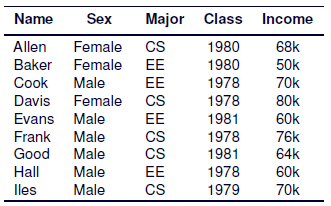
\includegraphics[scale=0.6]{img/statdbms.png}
\end{center}
Query 1: somma degli income degli individui con major EE (il risultato non espone nessun individuo)\\
Query 2: somma degli income dei maschi con major EE (il risultato non espone nessun individuo)\\
Query 3: somma degli income delle femmine con major EE (il risultato espone Baker)\\
La combinazione di queste query è sensibile.

\subsection{Macrodata e protezione}
Come abbiamo visto in precedenza le tabelle di macrodati possono essere classificate come:
\begin{itemize}
    \item di conteggio/frequenza: ogni cella contiene il numero dei rispondenti che hanno una certa caratteristica
    \item di grandezza: ogni cella contiene un valore aggregato di una quantità di interesse.
\end{itemize}
Vediamo nel dettaglio ora qualche tecnica di protezione di questi tipi di tabelle.

\subsection{Tabelle di conteggio}
Tendenzialmente contengono dati provenienti da sondaggi. Le tecniche di protezione adottate includono:
\begin{itemize}
    \item sampling
    \item regole speciali
    \item regole soglia
\end{itemize}

\subsubsection{Sampling}
Conduciamo un sondaggio e ne pubblichiamo i risultati.\\
Le stime sono fatte moltiplicando la singola risposta con un sampling weight prima di aggregarli.\\
Se i pesi non sono pubblicati, questo processo rende meno identificabili gli individui. \\
Le stime devono raggiungere un'accuratezza specifica e i dati che non rispecchiano questi requisiti non vengono pubblicati.

\subsubsection{Regole speciali}
Quando vengono definite tabelle di macrodati su tutta la popolazione devono essere effettuate delle limitazioni nelle divulgazioni. Le \textbf{regole speciali} definiscono restrizioni sul livello di dettaglio che può fornire una determinata tabella. Queste regole differiscono in base a organizzazioni e tipi di tabelle.\\
Esempio: Le regole di SSA (Social Security Administration) proibiscono la pubblicazione di tabelle dove il valore di una cella:
\begin{itemize}
    \item è uguale a un totale marginale
    \item permette all'utente di determinare
    \begin{itemize}
        \item l'età di un individuo all'interno di un intervallo di 5 anni
        \item guadagni all'interno di 1000\$ di intervallo
        \item benefit all'interno di 50\$ di intervallo
    \end{itemize}
\end{itemize}
Consideriamo la tabella che segue con questa regola speciale: l'income non deve stare all'interno di un intervallo di 5k
\begin{center}
    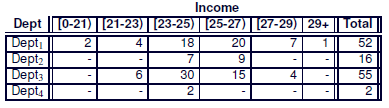
\includegraphics[scale=0.7]{img/sprules.png}
\end{center}
Questa tabella non potrebbe essere rilasciati per diversi motivi:
\begin{itemize}
    \item il valore di una cella è uguale al totale (\(Dept_4\))
    \item il valore di (\(Dept_2\)) ha dei rispondenti che stanno dentro ad un intervallo di income di 5K
\end{itemize}
Per ovviare a questo problema potrei ristrutturare la tabella e combinare righe e/o colonne, rendendola pubblicabile.

\subsubsection{Regole di soglia}
Una cella è sensibile se il numero di rispondenti è minore di un certo valore specificato. Quando abbiamo una cella sensibile questa non andrebbe mai rilasciata. Possiamo adottare diverse tecniche per proteggere celle sensibili:
\begin{itemize}
    \item ristrutturare la tabella e combinare le categorie
    \item soppressione di celle
    \item arrotondamento (casuale o controllato)
    \item modifica dei dati
\end{itemize}
Prendiamo come esempio la tabella che segue per spiegare le varie tecniche:
\begin{center}
    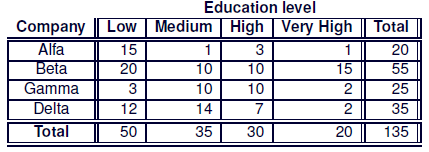
\includegraphics[scale=0.6]{img/regsog.png}
\end{center}
Questa tabella ha diversi valori sensibili (con numero di rispondenti \(<5\)).
\paragraph{Soppressione di celle}
È una delle tecniche più utilizzate, ma sopprimere le celle sensibili non è sufficiente (soppressione primaria) poichè il valore nella cella sensibile può essere calcolato dal totale marginale. Per rendere veramente sicuri i dati sensibili dobbiamo applicare una soppressione complementare dove viene soppressa almeno un'altra cella per ogni riga o colonna dove è stata già applicata la soppressione primaria. (Anche con la soppressione complementare è difficile garantire una protezione adeguata).\\
Per effettuare la soppressione complementare vengono usate techine lineari per selezionare quale cella dobbiamo sopprimere e successivamente vengono applicate tecniche di audit per valutare la bontà della soppressione applicata.\\
Il rischio della soppressione è quello di arrivare ad ottenere una tabella che ha più valori soppressi che valori pubblicati.
\begin{center}
    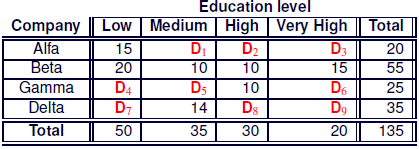
\includegraphics[scale=0.6]{img/supp.png}
\end{center}
\paragraph{Arrotondamento}
Per ridurre la perdita di dati dovuta alla soppressione possiamo introdurre un'approssimazione a un multiplo della soglia di sensibilità:
\begin{itemize}
    \item casuale: deicisioni casuali sull'arrotondamento per eccesso o difetto
    \begin{center}
        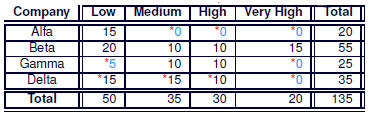
\includegraphics[scale=0.6]{img/randomround.png}
    \end{center}
    \item controllato: mi assicuro che le somme dei record siano uguali a quelle dei risultati totali marginali
    \begin{center}
        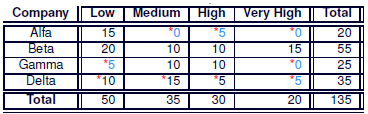
\includegraphics[scale=0.6]{img/contround.png}
    \end{center}
\end{itemize}
Anche in questo caso vengono utilizzati dei metodi di programmazione lineare per identificare l'approssimazione controllata di una tabella.\\
Questo metodo ha due svantaggi:
\begin{itemize}
    \item richiede l'utilizzo di programmi particolari
    \item non esiste sempre una soluzione per l'approssimazione controllata
\end{itemize}

\paragraph{Modifica dei dati}
Si modificano i dati alla base (microdati) e poi si calcolano le statistiche con i dati modificati (macrodati). Per applicare questa tecnica ovviamente devo conoscere lo scopo per cui questi dati vengono utilizzati per non "sporcare" eccessivamente e sballare le statistiche.\\
Questo è un metodo sviluppato dall' U.S. Census Bureau.\\
Il procedimento da loro applicato è:
\begin{enumerate}
    \item prendo un campione di record dai microdati
    \item trovo una corrispondenza per questi record in qualche altra area geografica, matchando su una serie di specificati attributi importanti
    \item swappo tutti gli attributi dei record matchati 
\end{enumerate}

\subsection{Tabelle di grandezza}
Solitamente sono tabelle che contengono la somma (non negativa) di qualcosa (ad esempio il fatturato di determinate aziende). Il nostro obiettivo è limitare le tecniche che si focalizzano sulla valutazione di stime precise dei valori.\\
Primary suppression rules determina quando un acella potrebbe rivelare l'individuo rispondete a quell'informazione. Tale cella viene considerata sensibile e non può essere rilasciata. Le suppression rules più comuni sono:
\begin{itemize}
    \item p-percent rule
    \item pq rule
    \item (n, k) rule
\end{itemize}
Queste rules vengono utilizzare per identificare le celle sensibili, verificando dove non è abbastanza difficile determinare una stima precisa di un valore di un rispondente.

\subsubsection{Soppressione primaria: p-percent}
La cella è esposta se si riesce a calcolare il valore del rispondente in maniera troppo accurata. Cosa significa “troppo accurata”? Se l’intervallo di stima (upper-lower) è più vicino al valore esatto rispetto a una percentuale p.\\
Più formalmente, una cella è protetta se:
\[\sum_{i=c+2}^N x_i \geq \frac{p}{100}x_1\]
dove\\ 
\(x_1,...,x_N\): sono i valori dei rispondenti in ordine decrescente \\
c: dimensione della coalizione di rispondenti "interpellati" cercando di stimare \(x_1\) \\
\(x_1\): valore più esposto \\

Esempio: consideriamo i rispondenti che contribuiscono all'entrata totale della città che è uguale a 250k
\begin{itemize}
    \item Alice: 100k
    \item Bob: 80k
    \item Carol: 30k
    \item David: 20k
    \item Eve: 10k
    \item Frank: 3k
\end{itemize}
Il valore più sensibile è quello di Alice poichè è il più facile da stimare. Quindi se proteggiamo il valore di Alice in modo che non possa essere stimato facilmente, anche tutti gli altri valori saranno protetti.\\
Qual è la coalizione di c = 3 rispondenti che possono stimare meglio l'entrata di Alice?\\
Bob, Carol, David, il quale ingresso è 130k, possono stimare che l'ingresso di Alice è tra gli 80K e i 120K (siccome deve essere maggiore o uguale degli 80k di Bob e minore uguale di 120k dateo che 250 - 130 = 120).\\
La cella è sensibile per ogni \(p \geq 20\) \\
Formalmente la cella è protetta per p con:
\[\sum_{i=c+2}^N x_i \geq \frac{p}{100}x_1\]
\[\sum_{i=3+2}^N x_i \geq \frac{p}{100}Alice\]
\[\sum_{i=5}^N x_i \geq \frac{p}{100}100\]
\[Cell - \sum_{i=c+2}^N x_i \geq p \]
\[Cell - (Alice + Bob + Carol + David) \geq p \]
\[250 - (100 + 80 + 30 + 20) \geq p \]
\[20 \geq p \]

\subsubsection{Soppressione primaria: pq rule}
Nel p-percent si assume che non ci siano conoscenze pregresse sui valori dei rispondenti e le agenzie non dovrebbero mai fare queste assunzioni.\\
Nel pq rule si può esprimere quanta conoscenza pregressa c'è assegnando un valore q che rappresenta quantro accuratamente il rispondente può stimare un valore di un altro rispondente prima che i dati vengano pubblicati \(( p < q < 100)\).\\
Formalmente una cella è protetta se: 
\[\frac{q}{100} \sum_{i=c+2}^N x_i \geq \frac{p}{100}x_1\]
dove\\ 
\(x_1,...,x_N\): sono i valori dei rispondenti in ordine decrescente \\
c: dimensione della coalizione di rispondenti "interpellati" cercando di stimare \(x_1\) \\
\(x_1\): valore più esposto \\
Se q=100 si assume che i rispondenti non sappiano nulla e non ci sia conoscenza a priori, la formula torna ad essere come quella di p-percent\\
Esempio: assumiamo che l'abilità di stimare il valore degli altri rispondenti sia q = 80\%.\\
Tutti sanno che l'entrata di Alice è tra 20k e 180k\\
Qual è la coalizione di c = 3 rispondenti che possono stimare meglio l'entrata di Alice?\\
Bob, Carol, David, possono ridurre l'incertezza e posizionare l'entrata di Alice tra 80K e i 120K (siccome deve essere maggiore o uguale degli 80k di Bob e minore uguale di 120k dateo che 250 - 130 = 120).\\
Formalmente la cella è protetta per p con:
\[\frac{q}{100} \sum_{i=c+2}^N x_i \geq \frac{p}{100}x_1\]
\[\frac{80}{100} \sum_{i=3+2}^N x_i \geq \frac{p}{100}Alice\]
\[\frac{80}{100} \sum_{i=5}^N x_i \geq \frac{p}{100}100\]
\[\frac{80}{100} \sum_{i=5}^N x_i \geq p\]
\[\sum_{i=5}^N x_i \geq \frac{p}{0.80}\]
\[Cell - \sum_{i=5}^N x_i \geq \frac{p}{0.80}\]
\[Cell - (Alice + Bob + Carol + David) \geq \frac{p}{0.80} \]
\[250 - (100 + 80 + 30 + 20) \geq \frac{p}{0.80} \]
\[20 \geq \frac{p}{0.80} \]
\[16 \geq p \]

\subsubsection{Soppressione primaria: (n, k) rule}
Riguarda il numero di rispondenti in una cella: se un numero piccolo (n o meno) di questi corrispondenti contribuisce ad una larga percentuale (k o più) del valore totale della cella, questa cella è considerata sensibile.\\
Se ci pensiamo è abbastanza intuitiva come regola, infatti: se una cella è dominata dal valore di un rispondente è facile capire che il totale è un valore che sovrastima il suo.\\
Solitamente si scelgono n = 1 o n = 2.\\

Esempio: supponiamo che con n = 2 e k = 70, la cella è considerata sensibile.\\
L'entrata di Alice e Bob è il 70\% del totale (180k su 250k).

\subsubsection{Soppressione secondaria}
Una volta che viene identificata una cella sensibile abbiamo due opzioni:
\begin{itemize}
    \item ristrutturare la tabella e collassare celle fino quando non rimangono più celle sensibili
    \item soppressione delle celle: non pubblichiamo cell sensibili (primary suppression) e rimuoviamo altre celle (complementary suppression)
\end{itemize}
Amministrativamente si può anche richiedere un consenso scritto dei rispondenti che li autorizzano a pubblicare certi dati.\\
Nonostante ciò possono essere rilasciate lo stesso delle celle sensibili visto che:
\begin{itemize}
    \item unioni implicite delle celle soppresse potrebbero essere sensibili
    \item l'equazione tra righe e colonne che viene rappresentata dalla tabella pubblicata potrebbe essere risolta
\end{itemize}

\paragraph{Audit} Per verificare che dopo la soppressione complementare non ci siano più celle sensibili vengono usate tecniche automatiche di audit.\\
Se vengono pubblicati i totali la somma delle celle soppresse potrebbe essere derivata. Applicando le regole di sensibilità a queste somme ci assicura che non siano sensibili:
\begin{itemize}
    \item righe e colonne possono essere visti come sistemi di equazioni lineari
    \item stimare un limite superiore o inferiore per ogni cella soppressa usando la programmazione lineare.
    \item se i margini sono troppo vicini al valore originale, la cella è sensibile
\end{itemize}
Tutto ciò è molto semplice per le tabelle piccole, mentre diventa computazionalmente intrattabile per tabelle grandi.

\paragraph{Perdita di informazioni} La selezione delle celle complementari deve risultare minima in termini di perdita di informazioni. Potremmo tentare di minimizzare:
\begin{itemize}
    \item la somma dei valori soppressi
    \item il numero totale di celle soppresse
\end{itemize}

Esempio: 
\begin{center}
    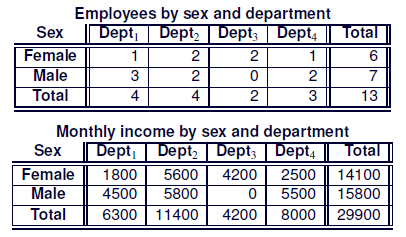
\includegraphics[scale=0.6]{img/magtab1.png}
\end{center}
Applichiamo a questa tabella (n, k) rule con n = 1 e k = 90, quindi una cella è sensibile se un rispondente contribuisce a più del 90\% del totale.\\
Ovviamente in questo caso sono Female / \(Dept_1\) e Female / \(Dept_4\) \\
Applicando soppressione primaria i valori di Female / \(Dept_1\) e Female / \(Dept_4\) sarebbero comunque ricavabili. Applicando invece la soppressione complementare otteniamo la tabella come segue, priva di celle sensibili:
\begin{center}
    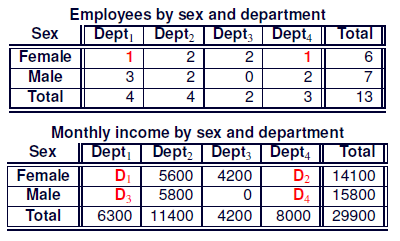
\includegraphics[scale=0.6]{img/magtab2.png}
\end{center}

\subsection{Microdati e protezione}
Molte situazioni richiedono il rilascio di dati specifici (microdati). Il vantaggio di pubblicare questo tipo di dato è la crescente flessibilità e disponibilità di informazioni.\\
Per proteggere l'anonimità del rispondente i data holder rimuovono o criptano spesso identificatori espliciti come nomi, indirizzi e num. di telefono. Ma questa operazione di deidentificazione dei dati non garantisce l'anonimità. Infatti il rilascio di dati quasi identificanti come lo ZIP, possono essere linkati insieme per risalire al rispondente.\\
Le strategie di protezione dei dati seguono essenzialmente due strategie:
\begin{itemize}
    \item ridurre il contenuto di informazioni
    \item cambiare i dati in maniera che l'informazione sia mantenuta il più possibile
\end{itemize}
Per proteggere i dati dal rischio di divulgazione si dovrebbe seguire la seguente procedura:
\begin{itemize}
    \item includere solo un campione di tutta la popolazione
    \item rimuovere gli identificatori
    \item limitazione dei dettagli geografici
    \item limitazione del numero di variabili 
\end{itemize}
Anche la locazione geografica è un dato sensibile da proteggere in quanto è sempre più spesso utilizzato nei microdati ed è identificante per il rispondente.\\
Le tecniche di protezione dei microdati sono basate sulla limitazione del processo di identificazione riducendo la quantità di informazioni rilasciate e possono essere divise in due categorie:
\begin{itemize}
    \item mascheramento dei dati: copro i dati non rilasciandoli o introducendo rumore
    \item sintetizzazione dei dati: rilascio dati non veri, ma plausibili
\end{itemize}
Queste tecniche possono operare su due tipi diversi di microdati:
\begin{itemize}
    \item continui: numerici e possiamo definire operazioni aritmetici su di essi
    \item categorici: possono assumere determinati e limitati valori e non possiamo eseguire operazioni aritmetiche su di essi
\end{itemize}

\subsection{Tecniche di mascheramento}
I dati originali vengono tasformati per produrre dei nuovi dati che sono validi per analisi statistiche e che mantengono inviolata la confidenzialità dei rispondenti. Queste tecniche di mascheramento si suddividono in:
\begin{itemize}
    \item non perturbative: i dati originali non sono modificati, ma alcuni vengono soppressi o ne vegnono rimossi dei dettagli
    \item perturbative: i dati originali vengono modificati (introduciamo rumore)
\end{itemize}
Lista di tecniche:\\\\

\begin{tabular}{ |p{3cm}||p{3cm}|p{3cm}|  }
 \hline
 \multicolumn{3}{|c|}{Non perturbative} \\
 \hline
Tecnica & Continui & Categorici \\
 \hline
Sampling & sì & sì  \\
Local Suppression & sì & sì  \\
Global Recoding & sì & sì  \\
Top-coding & sì & sì  \\
Bottom-coding & sì & sì  \\
Generalization & sì & sì  \\
 \hline
\end{tabular}

\begin{tabular}{ |p{3cm}||p{3cm}|p{3cm}|  }
 \hline
 \multicolumn{3}{|c|}{Perturbative} \\
 \hline
Tecnica & Continui & Categorici \\
 \hline
Resampling & sì & no  \\
Lossy Compression & sì & no  \\
Rounding & sì & no  \\
PRAM & no & sì  \\
MASSC & no & sì  \\
Random Noise & sì & sì  \\
Swapping & sì & sì  \\
Rank Swapping & sì & sì  \\
Micro-aggregation & sì & sì  \\
 \hline
\end{tabular}

\subsubsection{Sampling}
Per proteggere la tabella pubblico solo un campione dei microdati, riducendo così il rischio di re identificazione. (Al posto che pubblicare 14 tuple, ne pubblico 11)

\subsubsection{Local Suppression}
Questa tecnica sopprime il valore di un attributo (sostituendolo con un valore vuoto) che risulta significante per la re identificazione, limitando anche la possibilità di fare analisi.

\subsubsection{Global Recoding}
Il dominio di un attributo viene partizionato in intervalli disgiunti (di solito della stessa dimensione) identificati da un'etichetta. Per proteggere i dati quindi viene sostituito il valore di quest'attributo con la sua corrispondente etichetta.
\begin{center}
    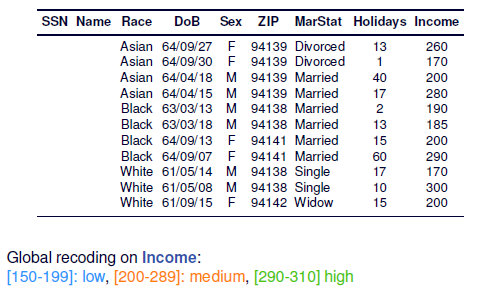
\includegraphics[scale=0.5]{img/globrec1.png}
\end{center}
\begin{center}
    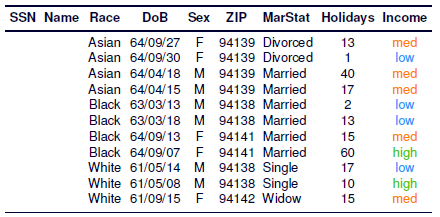
\includegraphics[scale=0.5]{img/globrec2.png}
\end{center}

\subsubsection{Top-coding e Bottom-Coding}
Top-coding definisce un limite superiore (top-code) entro in quale un valore deve stare. Se il valore di un attributo sfora questo limite il suo valore viene rimpiazzato con top-code.\\\\
Bottom-coding definisce un limite inferiore (bottom-code) entro in quale un valore deve stare. Se il valore di un attributo sfora questo limite il suo valore viene rimpiazzato con bottom-code.
\begin{center}
    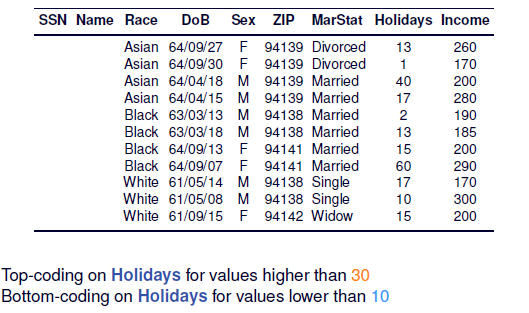
\includegraphics[scale=0.5]{img/topbott1.png}
\end{center}
\begin{center}
    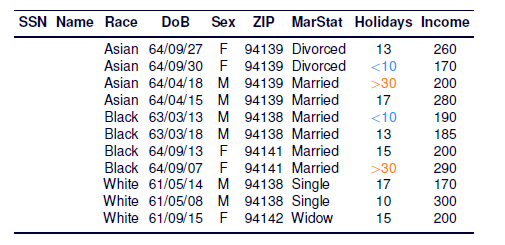
\includegraphics[scale=0.5]{img/topbott2.png}
\end{center}

\subsubsection{Generalization}
Consiste nel rappresentare un valore di un dato attributo usando dei valori più generici. È basato sulla definizione di una gerarchia di generalizzazione, dove il valore più generico è la radice e le foglie sono i valori più specifici.\\
Possono essere create diverse tabelle di microdati in base al livello di generalizzazione.

\subsubsection{Random noise}
Perturba i dati sensibili aggiungendo o moltiplicando il valore con una variabile random con una data distribuzione. Pubblicare questa distribuzione aumenta il rischio di divulgazione dei dati.

\subsubsection{Swapping}
Vengono scambiati i valori degli attributi di una piccola parte dei record che matchano con altri record nella stessa tabella (ossia sono molto simili).

\subsubsection{Micro-aggregation (blurring)}
Consiste nel raggruppare tuple in piccoli aggregati di dimensione k. \\ 
Al posto che pubblicare i singoli valori degli individui si pubblica una media del gruppo. Questi gruppi vengono formati utilizzando criteri di massima similtà.
\begin{center}
    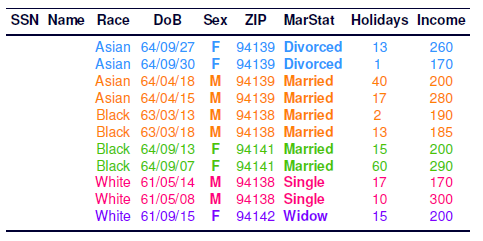
\includegraphics[scale=0.5]{img/blurring1.png}
\end{center}
Raggruppiamo le tuple in base a Sex e MartStat. Calcoliamo la media delle entrate per ogni gruppo e la sostituiamo con il valore dei singoli:
\begin{center}
    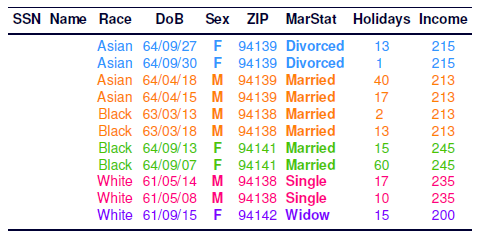
\includegraphics[scale=0.5]{img/blurring2.png}
\end{center}
\subsection{Tecniche sintetiche}
Siccome il contenuto statistico dei dati non è correlato alle informazioni date da ogni rispondente possiamo costruire un modello che rappresenta e sostituisce i dati forniti. \\
La cosa importante quando si costruiscono dati sintetici è che i dati originali e quelli sintetici devono fornire la stessa qualità di analisi statistica.\\
Il vantaggio principale di questa classe di tecniche è che i dati non sono correlati a nessun rispondente e quindi non può essere effettuata la re identificazione.
Lista di tecniche:\\\\

\begin{tabular}{ |p{3cm}||p{3cm}|p{3cm}|  }
 \hline
 \multicolumn{3}{|c|}{Totalmente sintetiche} \\
 \hline
Tecnica & Continui & Categorici \\
 \hline
Bootstrap & sì & no  \\
Cholesky Decomposition & sì & no  \\
Multiple Imputation & sì & sì  \\
Maximum Entropy & sì & sì  \\
Latin Hypercube Sampling & sì & sì  \\
 \hline
\end{tabular}

\begin{tabular}{ |p{3cm}||p{3cm}|p{3cm}|  }
 \hline
 \multicolumn{3}{|c|}{Parzialmente sintetiche} \\
 \hline
Tecnica & Continui & Categorici \\
 \hline
IPSO & sì & no  \\
Hybrid Masking & sì & no  \\
Random Response & no & sì \\
Blank and Impute & sì & sì  \\
SMIKe & sì & sì  \\
Multiply Imputed Partially Synthetic Dataset & sì & sì  \\
 \hline
\end{tabular}